\documentclass[main.tex]{subfiles}
\newcommand{\DiagramaEscala}{0.9}
\begin{document}

\section{Diferenciación e Integración Numérica}

%--------------------------------------------------
% Diapositiva 1
%--------------------------------------------------

%--- Diapositiva: Motivación ---
\begin{frame}{Introducción}
  El cálculo es la matemática del cambio. Los ingenieros tratan continuamente con sistemas y procesos que cambian, por lo tanto, el cálculo es esencial.
  \begin{itemize}
    \item La diferenciación y la integración son conceptos fundamentales.
    \item La derivada representa la razón de cambio.
    \item La integral representa la suma acumulada.
  \end{itemize}
\end{frame}

%--- Diapositiva: Definición de derivada ---
\begin{frame}{Definición de derivada}
  \begin{block}{Aproximación por diferencias}
    \[ \frac{dy}{dx} = \lim_{\Delta x \to 0} \frac{f(x + \Delta x) - f(x)}{\Delta x} \]
  \end{block}
  Representa la pendiente de la recta tangente a la curva en un punto.
\end{frame}

%--- Diapositiva: Segunda derivada y derivadas parciales ---
\begin{frame}{Segunda derivada y derivadas parciales}
  \begin{itemize}
    \item Segunda derivada: mide la curvatura o rapidez de cambio de la pendiente.
    \item Derivadas parciales: se derivan funciones de múltiples variables, manteniendo constantes las demás.
  \end{itemize}
\end{frame}

%--- Diapositiva: Integración ---
\begin{frame}{Integración}
  \begin{block}{Definición}
    \[ \int_a^b f(x) \, dx \]
  \end{block}
  Representa el área bajo la curva entre \( x = a \) y \( x = b \).
  \begin{itemize}
    \item Acumulación de cantidades.
    \item El símbolo \( \int \) proviene de la letra S de suma.
  \end{itemize}
\end{frame}

%--- Diapositiva: Diferenciación e integración numérica ---
\begin{frame}{Diferenciación e integración numérica}
  \begin{itemize}
    \item Funciones complicadas o datos tabulados requieren métodos aproximados.
    \item Se utilizan diferencias finitas para derivadas y cuadratura para integrales.
    \item Los métodos gráficos eran comunes antes de las computadoras.
  \end{itemize}
\end{frame}

%--- Diapositiva: Aplicaciones en ingeniería ---
\begin{frame}{Aplicaciones en ingeniería}
  \begin{itemize}
    \item Ley de Newton: \( F = ma = m \frac{d^2x}{dt^2} \)
    \item Ley de Fourier: \( q = -k \frac{dT}{dx} \)
    \item Evaluación de áreas, promedios, masas, flujos, etc.
  \end{itemize}
\end{frame}

%--- Diapositiva: Regla del promedio (media) ---
\begin{frame}{Cálculo del promedio de una función continua}
  \begin{block}{Fórmula}
    \[ \text{Media} = \frac{1}{b - a} \int_a^b f(x) \, dx \]
  \end{block}
  Similar al promedio discreto, pero para funciones continuas.
\end{frame}

%--- Diapositiva: Integrales en varias dimensiones ---
\begin{frame}{Integrales en varias dimensiones}
  \begin{itemize}
    \item Integral de volumen: \( \int\int\int_V c(x,y,z) \, dx\,dy\,dz \)
    \item Integral de área: \( \int\int_A f(x,y) \, dx\,dy \)
    \item Casos como masa total, transferencia de calor, etc.
  \end{itemize}
\end{frame}

%--- Diapositiva: Conclusión y continuidad ---
\begin{frame}{Conclusión}
  \begin{itemize}
    \item Diferenciación e integración son pilares del análisis ingenieril.
    \item Métodos numéricos permiten trabajar con datos reales y funciones complejas.
    \item Se explorarán técnicas como: regla del trapecio, Simpson, Romberg y más.
  \end{itemize}
\end{frame}
%--- Diapositiva: Fórmulas de Newton-Cotes ---
\begin{frame}{Fórmulas de integración de Newton-Cotes}
  \begin{itemize}
    \item Aproximan una función por un polinomio: \( f(x) \approx a_0 + a_1x + \ldots + a_nx^n \).
    \item Se integran estos polinomios en lugar de la función original.
    \item Existen fórmulas \textbf{cerradas} (conocidos los extremos) y \textbf{abiertas} (sin extremos).
  \end{itemize}
\end{frame}

%--- Diapositiva: Regla del trapecio ---
\begin{frame}{Regla del trapecio}
  \begin{block}{Fórmula}
    \[ I \approx \frac{b - a}{2} [f(a) + f(b)] \]
  \end{block}
  Aproxima el área bajo la curva con el área de un trapecio.
  \begin{itemize}
    \item Altura promedio: \( \frac{f(a) + f(b)}{2} \)
    \item Ancho: \( b - a \)
  \end{itemize}
\end{frame}
%--- Diapositiva: Regla del trapecio paso a paso ---
\begin{frame}{Regla del trapecio: Paso a paso}
\textbf{Paso 1:} Aproximar \( f(x) \) con una línea recta entre \( x = a \) y \( x = b \):
\[ f(x) = f(a) + \frac{f(b) - f(a)}{b - a}(x - a) \]
\textbf{Paso 2:} Integrar esa recta entre \( a \) y \( b \):
\[ \int_a^b f(x) \, dx = \int_a^b \left[ f(a) + \frac{f(b) - f(a)}{b - a}(x - a) \right] dx \]
\textbf{Paso 3:} Resolver la integral:
\[ \int_a^b f(x) \, dx = (b - a) \cdot \frac{f(a) + f(b)}{2} \]
Este es el resultado final de la \textbf{regla del trapecio}.
\end{frame}
%--- Diapositiva: Error estimado desde interpolación ---
\begin{frame}{Obtención y error estimado desde interpolación de Newton}
\textbf{Paso 1:} Considerar el polinomio de interpolación hacia adelante de Newton-Gregory con término de error:
\[ f(x) = f(a) + s\Delta f(a) + \frac{s(s-1)}{2} \Delta^2 f(a) \]
Donde \( s = \frac{x - a}{h} \), \( dx = h\,ds \).

\textbf{Paso 2:} Sustituir en la integral:
\[ \int_a^b f(x)\,dx = h \int_0^1 \left[f(a) + s\Delta f(a) + \frac{s(s - 1)}{2} \Delta^2 f(a)\right] ds \]
\end{frame}

\begin{frame}
    
\textbf{Paso 3:} Evaluar la integral:
\[ I = h \left[ f(a) + \frac{1}{2} \Delta f(a) + \frac{1}{6} \Delta^2 f(a) \right] \]

Si se asume que \( \Delta^2 f(a) \approx h^2 f''(\xi) \), se obtiene:
\[ I = h \cdot \frac{f(a) + f(b)}{2} - \frac{h^3}{12} f''(\xi) \]

\textbf{Resultado final:}
\begin{block}{Regla del trapecio con término de error}
\[ I = \frac{h}{2} [f(a) + f(b)] - \frac{(b - a)^3}{12} f''(\xi) \]
\end{block}
\end{frame}
%--- Diapositiva: Error en la regla del trapecio ---
\begin{frame}{Error en la regla del trapecio}
  \begin{block}{Error de truncamiento local}
    \[ E_t = -\frac{(b - a)^3}{12} f''(\xi) \quad \text{con } \xi \in [a,b] \]
  \end{block}
  \begin{itemize}
    \item Si \( f(x) \) es lineal, el error es cero.
    \item Si \( f''(x) \neq 0 \), el error depende de la curvatura.
  \end{itemize}
\end{frame}

%--- Diapositiva: Conclusión ---
\begin{frame}{Conclusión}
  \begin{itemize}
    \item Newton-Cotes permite integrar funciones complejas con polinomios.
    \item La regla del trapecio es el caso más simple.
    \item Se analizarán reglas más precisas como Simpson 1/3 y 3/8.
  \end{itemize}
\end{frame}

%--- Diapositiva: Ejemplo 21.1 (1/3) ---
\begin{frame}{Ejemplo 21.1: Paso a paso (1/3)}
\textbf{Función:}
\[ f(x) = 0.2 + 25x - 200x^2 + 675x^3 - 900x^4 + 400x^5 \]

\textbf{Intervalo:} \( a = 0, \; b = 0.8 \) \( \Rightarrow h = b - a = 0.8 \)

\textbf{Paso 1: Evaluar la función en los extremos}
\[ f(0) = 0.2 \]
\[ f(0.8) = 0.2 + 25(0.8) - 200(0.8)^2 + 675(0.8)^3 - 900(0.8)^4 + 400(0.8)^5 \]
\[ f(0.8) = 0.2 + 20 - 128 + 345.6 - 368.64 + 131.072 = 0.232 \]
\end{frame}

%--- Diapositiva: Ejemplo 21.1 (2/3) ---
\begin{frame}{Ejemplo 21.1: Paso a paso (2/3)}
\textbf{Paso 2: Aplicar la regla del trapecio}
\[ I \approx \frac{h}{2} [f(a) + f(b)] = \frac{0.8}{2} (0.2 + 0.232) \]
\[ I = 0.4 (0.432) = 0.1728 \]

\textbf{Paso 3: Calcular el error verdadero}
\[ I_{exacta} = 1.640533 \Rightarrow E_t = 1.640533 - 0.1728 = 1.467733 \]
\[ \epsilon_t = \frac{1.467733}{1.640533} \times 100\% \approx 89.5\% \]

\textbf{Conclusión:} La regla del trapecio subestima el área por la curvatura de la función.
\end{frame}

%--- Diapositiva: Ejemplo 21.1 (3/3): Gráfica con TikZ ---
\begin{frame}{Ejemplo 21.1: Visualización gráfica con TikZ}
\begin{center}
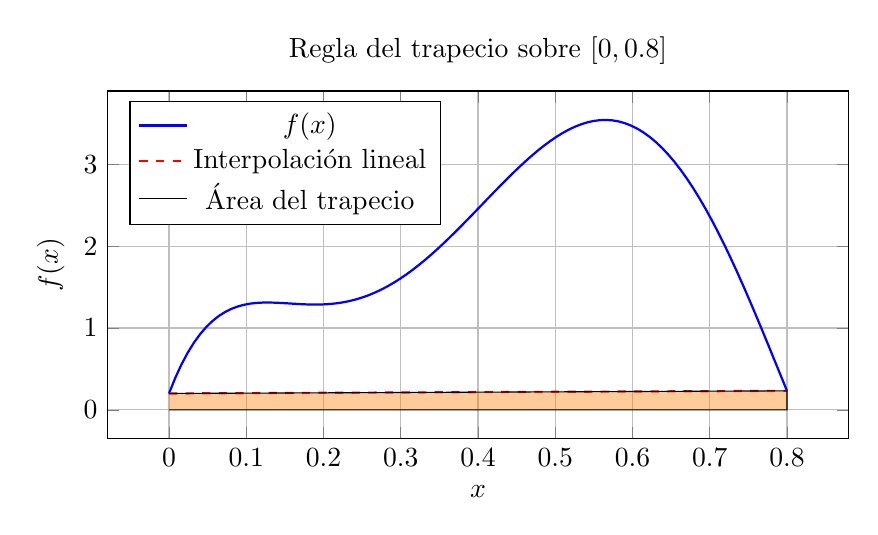
\begin{tikzpicture}
  \begin{axis}[
    width=11cm, height=6cm,
    domain=0:0.8,
    samples=100,
    xlabel={$x$}, ylabel={$f(x)$},
    grid=both, legend pos=north west,
    title={Regla del trapecio sobre $[0, 0.8]$}
  ]
    \addplot[blue, thick] {0.2 + 25*x - 200*x^2 + 675*x^3 - 900*x^4 + 400*x^5};
    \addlegendentry{$f(x)$}

    \addplot[red, dashed, thick, domain=0:0.8] {0.2 + (0.232 - 0.2)/0.8 * x};
    \addlegendentry{Interpolación lineal}

    \addplot[fill=orange, fill opacity=0.4] coordinates {(0,0.2) (0.8,0.232) (0.8,0) (0,0)};
    \addlegendentry{Área del trapecio}
  \end{axis}
\end{tikzpicture}
\end{center}
\end{frame}

%--- Diapositiva: Estimación detallada del error ---
\begin{frame}{Ejemplo 21.1: Estimación detallada del error}
\[ f''(x) = -400 + 4050x - 10800x^2 + 8000x^3 \]

\textbf{Paso 2: Cálculo del valor promedio de } \( f''(x) \) en \( [0, 0.8] \)
\begin{align*}
\text{Integrar: } & \int_0^{0.8} f''(x) dx \\
=\ & \int_0^{0.8} \left(-400 + 4050x - 10800x^2 + 8000x^3\right) dx \\
=\ & \left[-400x + \frac{4050}{2}x^2 - \frac{10800}{3}x^3 + \frac{8000}{4}x^4\right]_0^{0.8} \\
=\ & -320 + 1296 - 1536 + 409.6 = -150.4
\end{align*}

\textbf{Promedio:}
\[ f''_{prom} = \frac{-150.4}{0.8} = -188 \]
\end{frame}

%--- Diapositiva: Cálculo del error aproximado ---
\begin{frame}{Ejemplo 21.1: Cálculo del error aproximado}
\textbf{Paso 3: Sustituir en la fórmula del error estimado}
\[ E_a = -\frac{(b - a)^3}{12} f''_{prom} \]
\[ E_a = -\frac{(0.8)^3}{12} (-188) = \frac{0.512}{12} (188) = 8.021 \]

\textbf{Comparación:}
\begin{itemize}
  \item \( E_t = 1.640533 - 0.1728 = 1.467733 \)
  \item \( E_a = 8.021 \) sobrestima el error porque \( f''(x) \) tiene alta variabilidad.
  \item La suposición de derivada constante no es válida para funciones con mucha curvatura.
\end{itemize}
\end{frame}



%--- Diapositiva: Regla del trapecio compuesta ---
\begin{frame}{Regla del trapecio de aplicación múltiple}
\begin{itemize}
  \item Se divide \([a, b]\) en \(n\) subintervalos de igual tamaño.
  \item Se generan los nodos: \(x_0, x_1, x_2, \ldots, x_n\).
  \item La longitud de cada subintervalo es: \( h = \frac{b - a}{n} \).
\end{itemize}

\textbf{Paso 2: Aplicación de la regla del trapecio en cada subintervalo}
\[ I_i = \frac{h}{2} \left[ f(x_i) + f(x_{i+1}) \right] \]

\textbf{Paso 3: Suma total de áreas}
\[ I \approx \sum_{i=0}^{n-1} I_i = \frac{h}{2} \left[ f(x_0) + 2\sum_{i=1}^{n-1} f(x_i) + f(x_n) \right] \]

\textbf{Fórmula final:}
\[ I \approx \frac{b - a}{2n} \left[ f(x_0) + 2\sum_{i=1}^{n-1} f(x_i) + f(x_n) \right] \]
\end{frame}

%--- Diapositiva: Observaciones sobre el error compuesto ---
\begin{frame}{Error en la regla del trapecio compuesta}
\textbf{Error acumulado:}
\[ E = -\sum_{i=1}^n \frac{h^3}{12} f''(\xi_i) \]

\textbf{Estimación con derivada promedio:}
\[ E \approx -\frac{(b - a)^3}{12n^2} f''_{prom} \]

\textbf{Conclusiones:}
\begin{itemize}
  \item El error disminuye proporcionalmente a \( \frac{1}{n^2} \).
  \item Doblar los subintervalos reduce el error a la cuarta parte.
  \item La fórmula es válida bajo la suposición de derivada segunda continua.
\end{itemize}
\end{frame}

%--- Diapositiva: Ejemplo 21.2 (parte 1) ---
\begin{frame}{Ejemplo 21.2: Aplicación múltiple - Parte 1}
\textbf{Problema:} Estimar
\[ \int_0^{0.8} f(x)\,dx \quad \text{con} \quad f(x) = 0.2 + 25x - 200x^2 + 675x^3 - 900x^4 + 400x^5 \]
usando la regla del trapecio con \(n = 2\) segmentos.

\textbf{Paso 1:} Definición del intervalo
\begin{itemize}
  \item Intervalo: \(a = 0\), \(b = 0.8\)
  \item Subintervalos: \(n = 2\), \(h = \frac{b - a}{n} = 0.4\)
  \item Nodos: \(x_0 = 0\), \(x_1 = 0.4\), \(x_2 = 0.8\)
\end{itemize}

\textbf{Paso 2:} Evaluación de la función en los nodos:
\begin{align*}
  f(0) &= 0.2 \\
  f(0.4) &= 2.456 \\
  f(0.8) &= 0.232
\end{align*}
\end{frame}

%--- Diapositiva: Ejemplo 21.2 (parte 2) ---
\begin{frame}{Ejemplo 21.2: Aplicación múltiple - Parte 2}
\textbf{Paso 3:} Aplicar la fórmula del trapecio compuesta:
\[ I \approx \frac{0.8}{4} [0.2 + 2\cdot2.456 + 0.232] = 0.2 (0.2 + 4.912 + 0.232) = 1.0688 \]

\textbf{Paso 4:} Error verdadero:
\begin{align*}
  E_t &= 1.640533 - 1.0688 = 0.57173 \\
  e_t &= \frac{0.57173}{1.640533} \times 100 \approx 34.9\%
\end{align*}

\textbf{Paso 5:} Error estimado:
\[ f''_{prom} = -60 \quad \Rightarrow \quad E_a = -\frac{(0.8)^3}{12 \cdot 2^2} (-60) = 0.64 \]
\end{frame}

% Diapositiva 1: Introducción general
\begin{frame}{Regla de Simpson 1/3}
\textbf{Motivación:} Se desea mejorar la aproximación de integrales usando polinomios de mayor grado.

\begin{itemize}
  \item Se reemplaza el integrando por un polinomio de segundo grado (parábola).
  \item Requiere tres puntos igualmente espaciados: $x_0 = a$, $x_1 = \frac{a + b}{2}$, $x_2 = b$.
  \item El método se denomina \textbf{Simpson 1/3} porque el paso $h$ se divide entre 3.
\end{itemize}
\end{frame}

% Diapositiva 2: Deducción con Lagrange
\begin{frame}{Interpolación de segundo grado con Lagrange}
\textbf{Paso 1:} Se construye el polinomio de Lagrange de segundo grado para $f(x)$:
\begin{align*}
  f_2(x) &= \ell_0(x) f(x_0) + \ell_1(x) f(x_1) + \ell_2(x) f(x_2) \\
  \ell_0(x) &= \frac{(x - x_1)(x - x_2)}{(x_0 - x_1)(x_0 - x_2)} \\
  \ell_1(x) &= \frac{(x - x_0)(x - x_2)}{(x_1 - x_0)(x_1 - x_2)} \\
  \ell_2(x) &= \frac{(x - x_0)(x - x_1)}{(x_2 - x_0)(x_2 - x_1)}
\end{align*}
\end{frame}

% Diapositiva 3: Sustitución en la integral
\begin{frame}{Sustitución en la integral}
\textbf{Paso 2:} Se sustituye el polinomio interpolante en la integral:
\begin{align*}
  I &= \int_{x_0}^{x_2} f_2(x) dx \\
    &= \int_{x_0}^{x_2} \left[ \ell_0(x) f(x_0) + \ell_1(x) f(x_1) + \ell_2(x) f(x_2) \right] dx
\end{align*}
\textbf{Paso 3:} Separar la integral término a término:
\begin{align*}
  I &= f(x_0) \int_{x_0}^{x_2} \ell_0(x) dx + f(x_1) \int_{x_0}^{x_2} \ell_1(x) dx + f(x_2) \int_{x_0}^{x_2} \ell_2(x) dx
\end{align*}
\end{frame}

% Diapositiva 4: Evaluación de integrales
\begin{frame}{Evaluación de las integrales de Lagrange}
\textbf{Paso 4:} Suponiendo nodos equiespaciados con $h = (b - a)/2$:
\begin{align*}
  \int_{x_0}^{x_2} \ell_0(x) dx &= \frac{h}{3} \\
  \int_{x_0}^{x_2} \ell_1(x) dx &= \frac{4h}{3} \\
  \int_{x_0}^{x_2} \ell_2(x) dx &= \frac{h}{3}
\end{align*}
\textbf{Paso 5:} Sustituir los resultados en la integral:
\begin{block}{Fórmula de Simpson 1/3}
\[ I = \frac{h}{3} \left[ f(x_0) + 4f(x_1) + f(x_2) \right] \]
\end{block}
\end{frame}

% Diapositiva 5: Alternativa de presentación y error
\begin{frame}{Forma alternativa y error de truncamiento}
\textbf{Forma alternativa:}
\[ I = \frac{b - a}{6} [f(a) + 4f((a + b)/2) + f(b)] \]

\textbf{Error de truncamiento:}
\[ E = -\frac{(b - a)^5}{2880} f^{(4)}(\xi) \quad \text{con } \xi \in (a, b) \]

\textbf{Observaciones:}
\begin{itemize}
  \item Más precisa que la regla del trapecio.
  \item Exacta para polinomios de hasta grado 3.
  \item Utiliza tres puntos equiespaciados.
\end{itemize}
\end{frame}

%--- Diapositiva: Ejemplo 21.4 - Parte 1 ---
\begin{frame}{Ejemplo 21.4: Aplicación de la regla de Simpson 1/3 - Parte 1}
\textbf{Problema:} Calcular
\[
\int_0^{0.8} f(x)\,dx, \quad \text{con} \quad f(x) = 0.2 + 25x - 200x^2 + 675x^3 - 900x^4 + 400x^5
\]
utilizando la \textbf{regla de Simpson 1/3}. El valor exacto de la integral es \(1.640533\).
\textbf{Paso 1:} Definición del intervalo y nodos
\begin{itemize}
  \item Intervalo: \(a = 0\), \(b = 0.8\)
  \item Nodos: \(x_0 = 0\), \(x_1 = 0.4\), \(x_2 = 0.8\)
  \item Longitud de subintervalo: \(h = (b - a)/2 = 0.4\)
\end{itemize}

\textbf{Paso 2:} Evaluación de la función en los nodos:
\begin{align*}
  f(0) &= 0.2 \\
  f(0.4) &= 2.456 \\
  f(0.8) &= 0.232
\end{align*}
\end{frame}

%--- Diapositiva: Ejemplo 21.4 - Parte 2 ---
\begin{frame}{Ejemplo 21.4: Aplicación de la regla de Simpson 1/3 - Parte 2}
\textbf{Paso 3:} Aplicar la fórmula de Simpson 1/3:
\[
I \approx \frac{0.8}{6} [f(0) + 4f(0.4) + f(0.8)] = \frac{0.8}{6} [0.2 + 4(2.456) + 0.232] = 1.367467
\]

\textbf{Paso 4:} Error verdadero:
\begin{align*}
  E_t &= 1.640533 - 1.367467 = 0.2730667 \\
  \epsilon_t &= \frac{0.2730667}{1.640533} \times 100 \approx 16.6\%
\end{align*}

\textbf{Paso 5:} Estimación del error:
\begin{align*}
  f^{(4)}_{\text{prom}} &= -2400 \\
  E_a &= -\frac{(0.8)^5}{2880} (-2400) = 0.2730667
\end{align*}
\textbf{Conclusión:} El resultado por Simpson es mucho más preciso que la regla del trapecio simple.
\end{frame}

%--- Diapositiva: Simpson 1/3 de aplicación múltiple - Parte 1 ---
\begin{frame}{Simpson 1/3 de aplicación múltiple - Parte 1}
\textbf{Motivación:} Mejorar la precisión dividiendo el intervalo \([a, b]\) en un número par de segmentos \(n\).

\textbf{Paso 1:} División del intervalo:
\begin{itemize}
  \item Intervalo \([a, b]\) dividido en \(n\) subintervalos \(\Rightarrow\) \(n+1\) puntos: \(x_0, x_1, \ldots, x_n\)
  \item Longitud del subintervalo: \(h = \frac{b - a}{n}\)
\end{itemize}

\textbf{Paso 2:} Aplicación de Simpson 1/3 a cada par de subintervalos:
\[
I_i = \frac{h}{3} [f(x_{2i}) + 4f(x_{2i+1}) + f(x_{2i+2})]
\]

\textbf{Paso 3:} Suma total:
\[
I \approx \frac{h}{3} \left[f(x_0) + 4\sum_{i=1, \text{impar}}^{n-1} f(x_i) + 2\sum_{i=2, \text{par}}^{n-2} f(x_i) + f(x_n)\right]
\]
\end{frame}

%--- Diapositiva: Simpson 1/3 de aplicación múltiple - Parte 2 ---
\begin{frame}{Simpson 1/3 de aplicación múltiple - Parte 2}
\textbf{Fórmula general:}
\[
I \approx \frac{b - a}{3n} \left[f(x_0) + 4\sum_{i=1,3,5}^{n-1} f(x_i) + 2\sum_{i=2,4,6}^{n-2} f(x_i) + f(x_n)\right]
\]

\textbf{Condiciones:}
\begin{itemize}
  \item El número de subintervalos \(n\) debe ser par.
  \item Los nodos deben estar igualmente espaciados.
\end{itemize}

\textbf{Estimación del error:}
\[
E = -\frac{(b - a)^5}{180 n^4} f^{(4)}(\xi), \quad \xi \in [a, b]
\]

\textbf{Conclusión:} Esta técnica mejora sustancialmente la precisión con respecto a la regla de Simpson simple, conservando eficiencia computacional.
\end{frame}

%--- Diapositiva: Ejemplo 21.5 - Parte 1 ---
\begin{frame}{Ejemplo 21.5: Simpson 1/3 de aplicación múltiple - Parte 1}
\textbf{Problema:} Estimar
\[ \int_0^{0.8} f(x)\,dx \quad \text{con} \quad f(x) = 0.2 + 25x - 200x^2 + 675x^3 - 900x^4 + 400x^5 \]
utilizando la fórmula de Simpson 1/3 compuesta con \(n = 4\). Valor exacto: \(1.640533\).

\textbf{Paso 1:} Definición de parámetros
\begin{itemize}
  \item Intervalo: \(a = 0\), \(b = 0.8\), \(n = 4\)
  \item Longitud del subintervalo: \(h = (b - a)/n = 0.2\)
  \item Nodos: \(x_0 = 0\), \(x_1 = 0.2\), \(x_2 = 0.4\), \(x_3 = 0.6\), \(x_4 = 0.8\)
\end{itemize}

\textbf{Paso 2:} Evaluación de la función:
\begin{align*}
  f(0) &= 0.2 & f(0.2) &= 1.288 \\
  f(0.4) &= 2.456 & f(0.6) &= 3.464 \\
  f(0.8) &= 0.232
\end{align*}
\end{frame}

%--- Diapositiva: Ejemplo 21.5 - Parte 2 ---
\begin{frame}{Ejemplo 21.5: Simpson 1/3 de aplicación múltiple - Parte 2}
\textbf{Paso 3:} Aplicación de la fórmula:
\[
I \approx \frac{0.8}{12} [f(0) + 4f(0.2) + 2f(0.4) + 4f(0.6) + f(0.8)]
\]
\[
= \frac{0.8}{12} [0.2 + 4(1.288) + 2(2.456) + 4(3.464) + 0.232] = 1.623467
\]

\textbf{Paso 4:} Error exacto:
\begin{align*}
  E_t &= 1.640533 - 1.623467 = 0.017067 \\
  \epsilon_t &= \frac{0.017067}{1.640533} \times 100 \approx 1.04\%
\end{align*}

\textbf{Paso 5:} Estimación del error:
\begin{align*}
  f^{(4)}_{\text{prom}} &= -2400 \\
  E_a &= -\frac{(0.8)^5}{180 \cdot 4^4} (-2400) \approx 0.017067
\end{align*}
\end{frame}
%--- Diapositiva: Regla de Simpson 3/8 ---
\begin{frame}{Regla de Simpson 3/8}
\textbf{Fundamento:} Ajustar un polinomio de Lagrange de tercer grado a cuatro puntos e integrarlo:
\[
I = \int_a^b f(x)dx \approx \frac{3h}{8}[f(x_0) + 3f(x_1) + 3f(x_2) + f(x_3)]
\]
\begin{itemize}
  \item \(h = \frac{b - a}{3}\)
  \item Cada subintervalo es igual y se requieren 4 puntos.
\end{itemize}
\textbf{Versión general:}
\[
I = \frac{3(b - a)}{8} [f(x_0) + 3f(x_1) + 3f(x_2) + f(x_3)]
\]
\textbf{Estimación del error:}
\[
E = -\frac{(b - a)^5}{6480} f^{(4)}(\xi), \quad \xi \in [a, b]
\]
\end{frame}

%--- Diapositiva: Observaciones sobre Simpson 3/8 ---
\begin{frame}{Observaciones sobre Simpson 3/8}
\textbf{Comparación:}
\begin{itemize}
  \item La regla 3/8 es más precisa que la regla 1/3 (denominador mayor en error).
  \item Requiere 4 puntos (3 subintervalos), mientras que la 1/3 sólo 3 puntos (2 subintervalos).
  \item Preferible usar Simpson 1/3 por simplicidad, salvo cuando el número de segmentos es impar.
\end{itemize}

\textbf{Ejemplo de combinación:}
\begin{itemize}
  \item Para 5 segmentos: usar Simpson 1/3 para los primeros 2 y 3/8 para los últimos 3.
  \item Así se mantiene precisión de tercer orden en todo el intervalo.
\end{itemize}

\textbf{Conclusión:} La regla 3/8 es útil en casos especiales donde Simpson 1/3 no es directamente aplicable.
\end{frame}
%--- Diapositiva: Ejemplo Regla de Simpson 3/8 ---
\begin{frame}{Ejemplo: Regla de Simpson 3/8 - Parte a}
\textbf{Problema:} Integrar \( f(x) = 0.2 + 25x - 200x^2 + 675x^3 - 900x^4 + 400x^5 \) en [0, 0.8] usando la regla de Simpson 3/8.

\textbf{Valores de la función:}
\begin{itemize}
  \item \( f(0) = 0.2 \)
  \item \( f(0.2667) = 1.432724 \)
  \item \( f(0.5333) = 3.487177 \)
  \item \( f(0.8) = 0.232 \)
\end{itemize}

\textbf{Resultado:}
\[
I \approx \frac{0.8}{8} [0.2 + 3(1.432724 + 3.487177) + 0.232] = 1.519170
\]
\textbf{Error verdadero:} \( Et = 1.640533 - 1.519170 = 0.121363 \Rightarrow et = 7.4\% \)
\end{frame}

%--- Diapositiva: Ejemplo combinado (Simpson 1/3 y 3/8) ---
\begin{frame}{Ejemplo: Simpson 1/3 + 3/8 - Parte b}
\textbf{Datos:} 5 segmentos con \( h = 0.16 \)
\begin{itemize}
  \item \( f(0) = 0.2 \), \( f(0.16) = 1.296919 \), \( f(0.32) = 1.743393 \)
  \item \( f(0.48) = 3.186015 \), \( f(0.64) = 3.181929 \), \( f(0.80) = 0.232 \)
\end{itemize}

\textbf{Paso 1: Regla de Simpson 1/3 en [0, 0.32]}
\[
I_1 \approx \frac{0.32}{6}[0.2 + 4(1.296919) + 1.743393] = 0.3803237
\]

\textbf{Paso 2: Regla de Simpson 3/8 en [0.32, 0.80]}
\[
I_2 \approx \frac{0.48}{8}[1.743393 + 3(3.186015 + 3.181929) + 0.232] = 1.264754
\]

\textbf{Integral total:} \( I = I_1 + I_2 = 1.645077 \)
\textbf{Error:} \( Et = 1.640533 - 1.645077 = -0.00454383 \Rightarrow et = -0.28\% \)
\end{frame}
\begin{frame}{Grafica}
\begin{center}
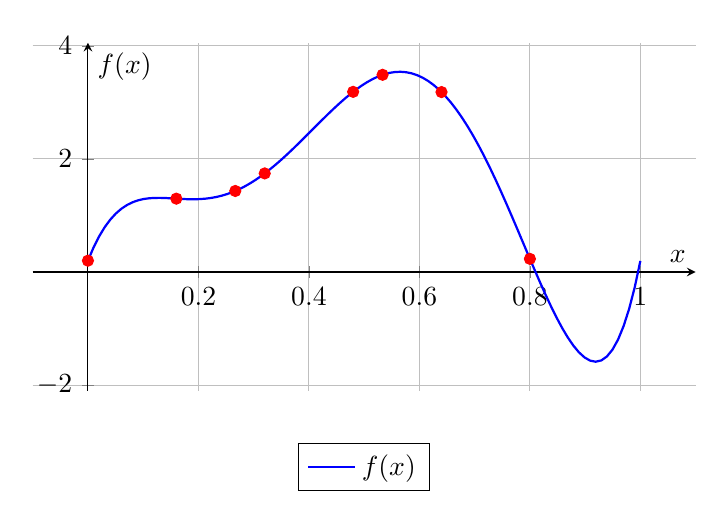
\begin{tikzpicture}
  \begin{axis}[
    width=10cm,
    height=6cm,
    axis lines=middle,
    xlabel={$x$}, ylabel={$f(x)$},
    domain=0:1,
    samples=100,
    grid=both,
    enlargelimits=true,
    clip=false,
    legend style={at={(0.5,-0.15)}, anchor=north}]
    \addplot [blue, thick] {0.2 + 25*x - 200*x^2 + 675*x^3 - 900*x^4 + 400*x^5};
    \addlegendentry{$f(x)$}
    \addplot[only marks, red, mark=*] coordinates {(0,0.2) (0.16,1.296919) (0.2667,1.432724) (0.32,1.743393) (0.48,3.186015) (0.5333,3.487177) (0.64,3.181929) (0.8,0.232)};
  \end{axis}
\end{tikzpicture}
\end{center}
\end{frame}


%--- Diapositiva: Algoritmos computacionales para reglas de Simpson ---
\begin{frame}{Algoritmos computacionales para las reglas de Simpson}
\textbf{Observaciones clave:}
\begin{itemize}
  \item Los algoritmos están diseñados para datos tabulados.
  \item Se requiere que los puntos estén igualmente espaciados.
  \item Deben evaluarse funciones conocidas o conocidas tabularmente.
\end{itemize}
\end{frame}

%--- Diapositiva: Tabla de Newton-Cotes ---
\begin{frame}{Tabla de reglas de Newton-Cotes}
\textbf{Fórmulas en formato general:}
\begin{center}
\scriptsize
\begin{tabular}{|c|c|c|c|}
\hline
Segmentos & Nombre & Fórmula & Error de truncamiento \\
\hline
1 & Trapecio & $\frac{b-a}{2}[f(x_0) + f(x_1)]$ & $-\frac{1}{12}h^3f''(\xi)$ \\
2 & Simpson 1/3 & $\frac{b-a}{6}[f(x_0) + 4f(x_1) + f(x_2)]$ & $-\frac{1}{90}h^5f^{(4)}(\xi)$ \\
3 & Simpson 3/8 & $\frac{b-a}{8}[f(x_0) + 3f(x_1) + 3f(x_2) + f(x_3)]$ & $-\frac{3}{80}h^5f^{(4)}(\xi)$ \\
\hline
\end{tabular}
\end{center}
\textbf{Donde:} $h = \frac{b - a}{n}$
\end{frame}



% Diapositiva 1: Introducción
\begin{frame}{Diferenciación numérica}
\begin{itemize}
  \item Las diferencias finitas permiten aproximar derivadas usando datos discretos.
  \item Las formas hacia adelante, hacia atrás y centradas se derivan de la serie de Taylor.
  \item Su exactitud depende del número de términos utilizados en la deducción.
  \item Se buscará aumentar la exactitud agregando términos adicionales.
\end{itemize}
\end{frame}

% Diapositiva 2: Serie de Taylor hacia adelante
\begin{frame}{Serie de Taylor hacia adelante}
\begin{equation*}
  f(x_i + h) = f(x_i) + f'(x_i) h + \frac{f''(x_i)}{2} h^2 + \cdots
\end{equation*}
\begin{itemize}
  \item De esta expresión se despeja:
\end{itemize}
\begin{equation*}
  f'(x_i) = \frac{f(x_i + h) - f(x_i)}{h} - \frac{f''(x_i)}{2}h + O(h^2)
\end{equation*}
\end{frame}

% Diapositiva 3: Aproximación mejorada
\begin{frame}{Aproximación mejorada con O(h$^2$)}
\begin{itemize}
  \item Usamos una estimación de $f''(x_i)$ con diferencias finitas:
\end{itemize}
\begin{equation*}
  f''(x_i) \approx \frac{f(x_i + 2h) - 2f(x_i + h) + f(x_i)}{h^2} + O(h)
\end{equation*}
\begin{itemize}
  \item Sustituyendo en la ecuación anterior:
\end{itemize}
\begin{equation*}
  f'(x_i) \approx \frac{-f(x_i + 2h) + 4f(x_i + h) - 3f(x_i)}{2h} + O(h^2)
\end{equation*}
\end{frame}
%--- Diapositiva: Ejemplo 23.1 Diferenciación con alta exactitud ---
\begin{frame}{Ejemplo 23.1: Estimación de la derivada}
\textbf{Función:}
\[f(x) = -0.1x^4 - 0.15x^3 - 0.5x^2 - 0.25x + 1.2\]

\textbf{Punto de evaluación:} $x = 0.5$, $h = 0.25$

\begin{itemize}
  \item \textbf{Derivada exacta:} $f'(0.5) = -0.9125$
  \item \textbf{Estimaciones:}
  \begin{itemize}
    \item Hacia adelante ($\mathcal{O}(h)$): $-1.155$ \quad $et = -26.5\%$
    \item Hacia atrás ($\mathcal{O}(h)$): $-0.714$ \quad $et = 21.7\%$
    \item Centrada ($\mathcal{O}(h^2)$): $-0.934$ \quad $et = -2.4\%$
  \end{itemize}
\end{itemize}

\textbf{Conclusión:} La fórmula centrada es mucho más precisa al ser de orden $\mathcal{O}(h^2)$.
\end{frame}

%--- Diapositiva: Tabla de fórmulas hacia adelante ---
\begin{frame}{Fórmulas hacia adelante: precisión creciente}
\begin{center}
\begin{tabular}{|c|l|c|}
\hline
\textbf{Orden} & \textbf{Fórmula} & \textbf{Error} \\
\hline
$f'(x_i)$ & $\frac{f(x_{i+1}) - f(x_i)}{h}$ & $\mathcal{O}(h)$ \\
$f'(x_i)$ & $\frac{-f(x_{i+2}) + 4f(x_{i+1}) - 3f(x_i)}{2h}$ & $\mathcal{O}(h^2)$ \\
\hline
$f''(x_i)$ & $\frac{f(x_{i+2}) - 2f(x_{i+1}) + f(x_i)}{h^2}$ & $\mathcal{O}(h)$ \\
$f''(x_i)$ & $\frac{-f(x_{i+3}) + 4f(x_{i+2}) - 5f(x_{i+1}) + 2f(x_i)}{h^2}$ & $\mathcal{O}(h^2)$ \\
\hline
$f'''(x_i)$ & $\frac{f(x_{i+3}) - 3f(x_{i+2}) + 3f(x_{i+1}) - f(x_i)}{h^3}$ & $\mathcal{O}(h)$ \\
$f'''(x_i)$ & $\frac{-3f(x_{i+4}) + 14f(x_{i+3}) - 24f(x_{i+2}) + 18f(x_{i+1}) - 5f(x_i)}{2h^3}$ & $\mathcal{O}(h^2)$ \\
\hline
$f^{(4)}(x_i)$ & $\frac{f(x_{i+4}) - 4f(x_{i+3}) + 6f(x_{i+2}) - 4f(x_{i+1}) + f(x_i)}{h^4}$ & $\mathcal{O}(h)$ \\
$f^{(4)}(x_i)$ & $\frac{-2f(x_{i+5}) + 11f(x_{i+4}) - 24f(x_{i+3}) + 26f(x_{i+2}) -14f(x_{i+1}) + 3f(x_i)}{h^4}$ & $\mathcal{O}(h^2)$ \\
\hline
\end{tabular}
\end{center}
\end{frame}
% Diapositiva 4: Comentarios finales
\begin{frame}{Comentarios finales}
\begin{itemize}
  \item La inclusión de términos adicionales mejora la exactitud de las derivadas numéricas.
  \item La expresión obtenida tiene error de truncamiento de orden $O(h^2)$.
  \item Se pueden desarrollar fórmulas análogas para diferencias centradas y hacia atrás.
\end{itemize}
\end{frame}

%--- Diapositiva: Derivadas parciales ---
\begin{frame}{Derivadas parciales: definiciones}
\textbf{Para funciones de dos variables: }$f(x,y)$
\begin{itemize}
  \item Las derivadas parciales de primer orden se calculan como:
  \[ \frac{\partial f}{\partial x} \approx \frac{f(x+\Delta x, y) - f(x - \Delta x, y)}{2\Delta x} \]
  \[ \frac{\partial f}{\partial y} \approx \frac{f(x, y+\Delta y) - f(x, y - \Delta y)}{2\Delta y} \]
  \item Se usan diferencias centradas, análogas a las univariadas.
\end{itemize}
\end{frame}

%--- Diapositiva: Derivadas parciales de segundo orden ---
\begin{frame}{Derivadas parciales de orden superior y mixtas}
\textbf{Derivadas parciales segundas y mixtas:}
\begin{itemize}
  \item Derivadas parciales segundas puras:
  \[ \frac{\partial^2 f}{\partial x^2} \approx \frac{f(x+\Delta x, y) - 2f(x,y) + f(x - \Delta x, y)}{\Delta x^2} \]
  \[ \frac{\partial^2 f}{\partial y^2} \approx \frac{f(x, y+\Delta y) - 2f(x,y) + f(x, y - \Delta y)}{\Delta y^2} \]
  \item Derivada parcial mixta:
  \[ \frac{\partial^2 f}{\partial x\partial y} \approx \frac{f(x + \Delta x, y + \Delta y) - f(x + \Delta x, y - \Delta y)}{2\Delta y} - \frac{f(x - \Delta x, y + \Delta y) - f(x - \Delta x, y - \Delta y)}{2\Delta y} \]
\end{itemize}
\end{frame}

%--- Diapositiva: Derivada parcial mixta simplificada ---
\begin{frame}{Aproximación final para derivada mixta}
Agrupando los términos anteriores, se obtiene:
\[ \frac{\partial^2 f}{\partial x \partial y} \approx \frac{f(x + \Delta x, y + \Delta y) - f(x + \Delta x, y - \Delta y) - f(x - \Delta x, y + \Delta y) + f(x - \Delta x, y - \Delta y)}{4\Delta x \Delta y} \]

\textbf{Conclusión:} Esta aproximación requiere 4 evaluaciones de la función alrededor del punto $(x,y)$ en una rejilla centrada.
\end{frame}
\end{document}